\documentclass[12pt,a4paper]{article}
\usepackage[utf8]{inputenc}
\usepackage[german]{babel}
\usepackage[T1]{fontenc}
\usepackage{amsmath}
\usepackage{amsfonts}
\usepackage{amssymb}
\usepackage{graphicx}
\usepackage[left=2.5cm,right=2.5cm,top=2cm,bottom=2cm]{geometry}
\author{Gruppe C14 \\ Julián Häck, Martin Koytek, Lars Wenning, Erik Zimmermann}
\usepackage{float}
\begin{document}
\section{Schallgeschwindigkeit in Festkörpern}
\subsection{Versuchsbeschreibung}
%Kurze Darstellung der physikalischen Grundlagen und Ziele der Versuche, die zum Verständnis des Versuches/Protokolls benötigt werden. (max. 1 Seite)
Die Ausbreitungsgeschwindigkeit v in einem Festkörper kann über den Elastizitätsmodul und die Dichte des Materials bestimmt werden:
\begin{equation}
v=\sqrt{\frac{E}{\rho}}
\end{equation}
Mit $v=f\cdot \lambda$ und $\lambda=2L$ ergibt sich für den Elastizitätsmodul:
\begin{equation}
E= \rho\cdot f^2\cdot 4L^2
\end{equation}

\subsection{Versuchsaufbau und Durchführung}
%Genaue Beschreibung der verwendeten Aufbauten unter Verwendung von Skizzen oder Photos
%Beschreibung der Messwerterfassungseinstellungen (eingestellte Messzeiten, Messbedingungen, Trigger, Anzahl der Messungen) und der Durchführung der Versuche. (max. 1 Seite)\newline
Zur Berechnung des Elastizitätsmoduls wurden 4 Stäbe mit Stativmaterial so eingespannt, dass diese nur in der Mitte einen Kontaktpunkt mit der Klemme haben (siehe Abbildung \ref{Stange}). Da wir dort einen Schwingunsknoten erwarten, können wir Verlusste durch die Aufhängung im Folgenden vernachlässigen. Nachdem wir die Massen der zylinderförmigen Stäbe bestimmt hatten und diese befestigt wurden, haben wir mehrfach die Dicken der Stangen an unterschiedlichen Stellen und die Längen gemessen. Des Weiteren konnten wir $\rho$ dann aus $\rho=\frac{M}{V}=\frac{4\cdot M}{L\cdot \pi D^2}$ bestimmen.\newline
Zur Messung der Eigenfrequenz haben wir auf das eine Stabende mit einem Gummihammer geschlagen, an dem anderen Ende wurde ein Mikrofon in ca. 5mm Entfernung angebracht, das wir mit Cassy verbunden haben. Dort konnten wir mittels Fast-Fourier-Transformation die Frequenzen bestimmen, wobei wir hier nur Grundschwingungen betrachtet haben.
\begin{figure}[H]
\centering
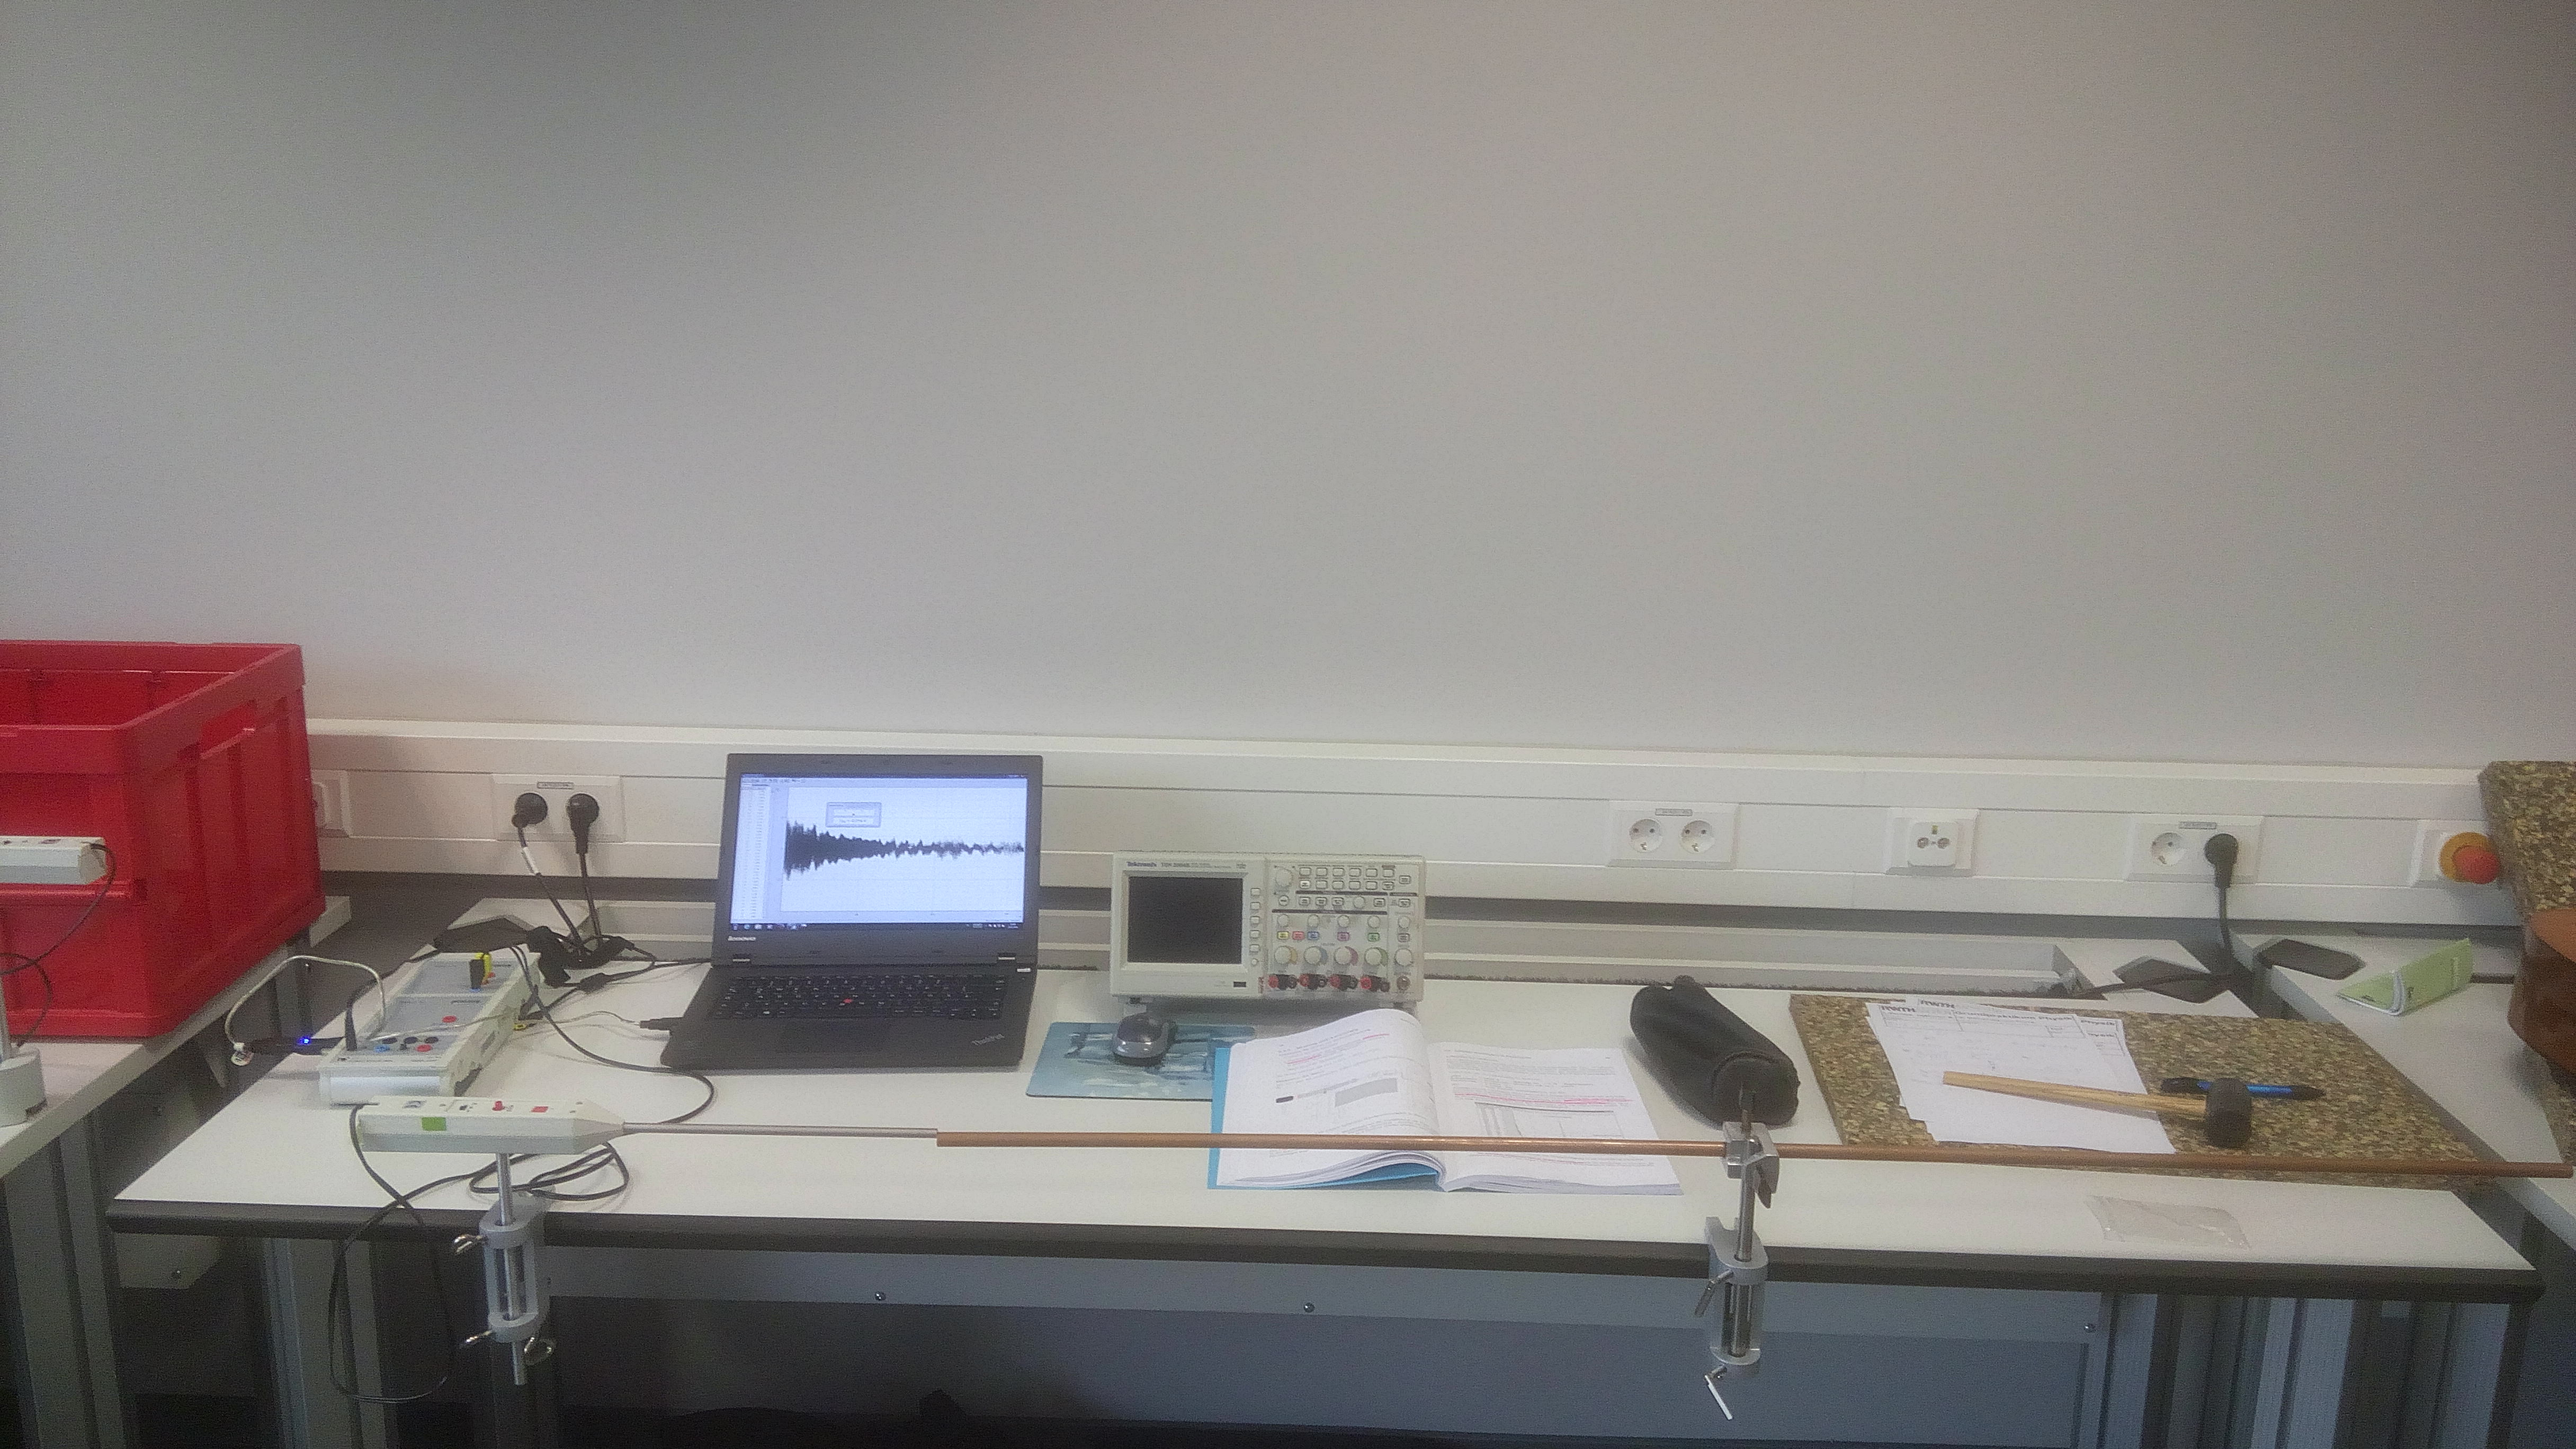
\includegraphics[scale=0.093]{Bilder/Arbeitsplatz_Stange.jpg}
\caption{Übersicht Arbeitsplatz}
\end{figure}

\begin{figure}[H]
\centering
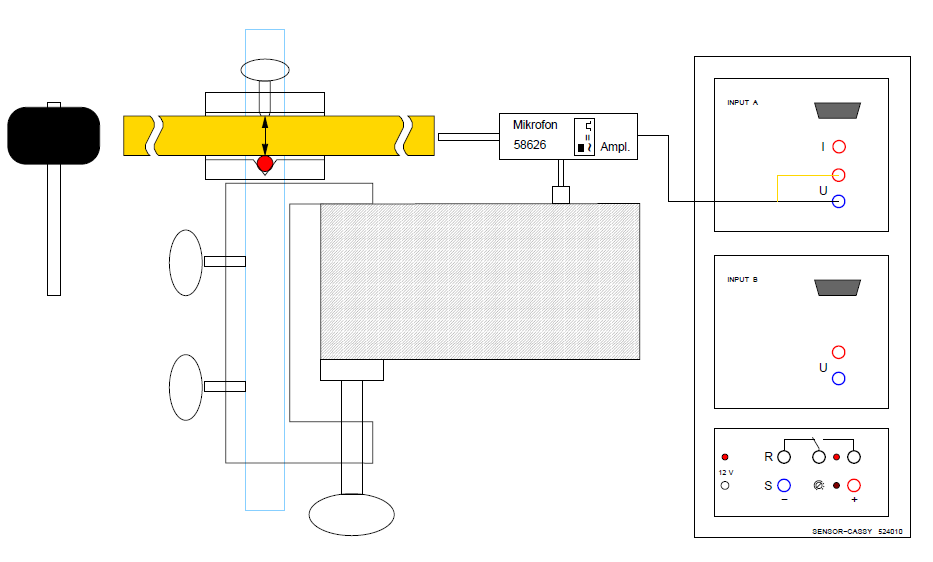
\includegraphics[scale=0.6]{Bilder/Versuchsaufbau_Skript.PNG}
\caption{Versuchsaufbau}
\label{Stange}
\end{figure}


\subsubsection{Messwerterfassungseinstellungen}
\begin{center}
\begin{tabular}{c|c}
Messbereich jeweils Messung 1-5 & -0.3..0.3V\\ 
\hline
Messbereich jeweils Messung 6-10 & -1.0..1.0V\\ 
\hline
Messintervall & 10$\mu$s \\ 
\hline
Messpunkte & 16000 \\ 
\hline
Messzeit & 1.6s \\ 
\end{tabular} 
\end{center}
Der Messbereich wurde hier immer nach der fünften Messung geändert, weil wir bei den Schlägen 6 bis 10 mit dem Stabende fester geschlagen haben und so die Amplituden in Cassy größer als der Messbereich wurden.
\subsubsection{Geräteübersicht}
\begin{itemize}
\item 4 Metallstangen
\item 1 Laptop
\item 1 Sensor-Cassy
\item 1 Universalmikrofon
\item 1 Gummi-Hammer
\item 1 Maßband
\item 1 Mikrometermaß
\item 1 Analysewaage
\item Stativzubehör
\end{itemize}
\newpage
\subsection{Versuchsauswertung}

\subsubsection{Rohdaten}

\begin{table}[H]\centering
\caption{Masse m und Länge L der Stangen}
\begin{tabular}{c|cccc}
& Stange 1 & Stange 2 & Stange 3 & Stange 4 \\ 
\hline
m in kg & 1.3019 & 1.3249 & 1.1570 & 1.2364 \\ 
L in m & 1.299  & 1.50 & 1.301 & 1.299 \\ 
\end{tabular} 
\end{table}
Der statistische Fehler auf die Einzelmessung ergibt sich zu:
\begin{align*}
\sigma_m=0.0001\,kg\\
\sigma_l=0.5\cdot10^{-2}\,m
\end{align*}
\begin{equation}
\sigma_i=\sqrt{\frac{\sum_i^n(x_i-x_{mean})^2}{n-1}}
\end{equation}

\begin{table}[H]\centering
\caption{Die Dicke d der Stangen (in mm) wurde an 5 verschiedenen Stellen gemessen.}
\begin{tabular}{c|cccc}
 & Stange 1 & Stange 2 & Stange 3 & Stange 4 \\ 
 \hline
$d_1$ & $12.47$ & $12.01$ & $11.97$ & $11.97$ \\ 
$d_2$ & $12.47$ & $12.00$ & $11.97$ & $11.97$ \\ 
$d_3$ & $12.47$ & $11.99$ & $11.95$ & $12.00$ \\ 
$d_4$ & $12.47$ & $11.99$ & $11.97$ & $11.97$ \\ 
$d_5$ & $12.47$ & $12.01$ & $11.96$ & $11.98$ \\ 
\hline
$d_{mean}$ & $12.47$ & 12.00 & 11.96 & 1198 \\ 
$\sigma_{d_{mean}}$ & $0.00$ & $4.47\cdot 10^{-3}$ & $4.00\cdot 10^{-3}$ & $5.83\cdot 10^{-3}$ \\ 
\end{tabular} 
\end{table}

Die Frequenzen f (in Hz) wurden mittels Fast-Fourier-Transformation und Peakschwerpunktbestimmung aus Cassy abgelesen.

\begin{figure}[H]
\centering
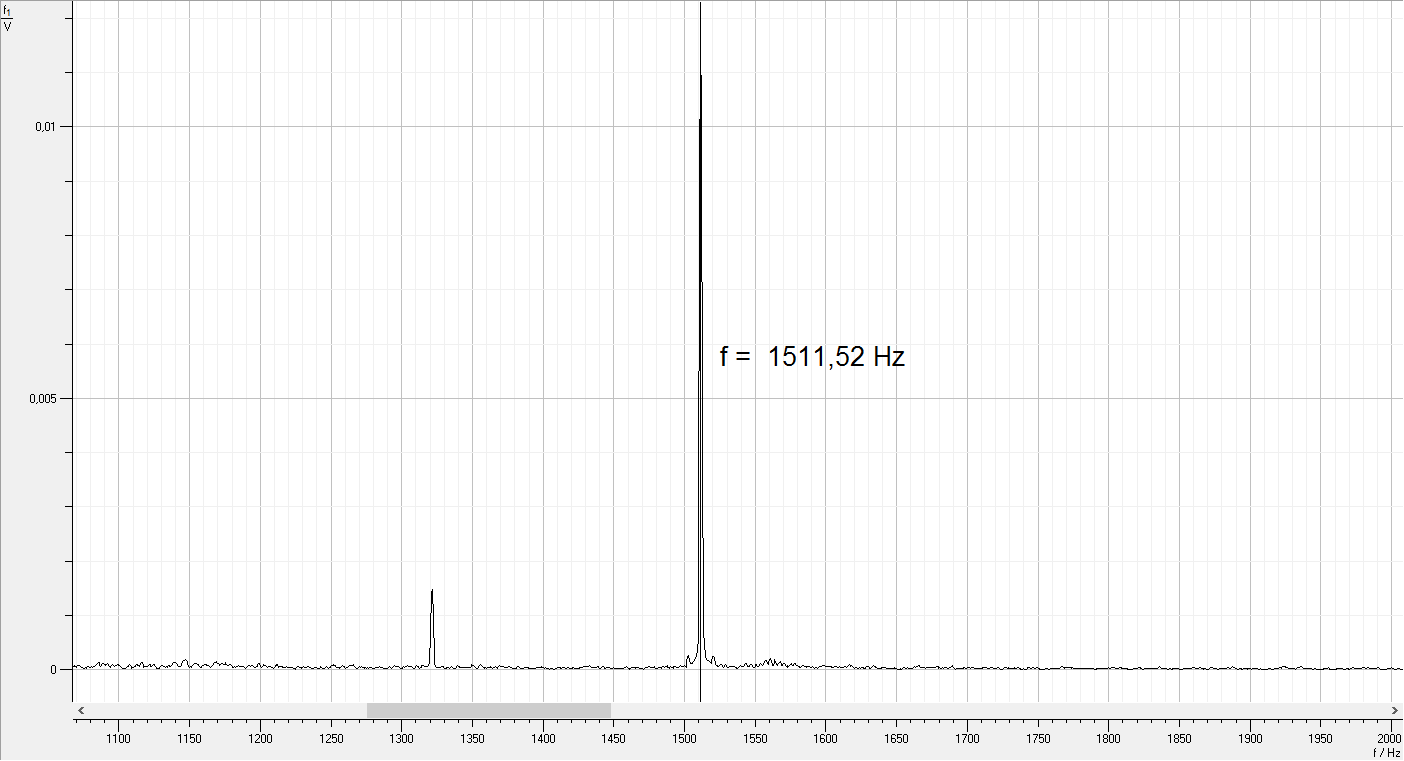
\includegraphics[scale=0.43]{Bilder/Beispiel_Cassy_Cu.png}
\caption{Beispiel zu Frequenz aus FFT ablesen (Stange 1)}
\end{figure}

\begin{table}[H]\centering
\caption{Frequenzen aus der FFT für alle 4 Stangen}
\begin{tabular}{c|cccc}
 & Stange 1 & Stange 2 & Stange 3 & Stange 4 \\ 
 \hline
$f_1$ & 1511.52 & 1728.17 & 1884.03 & 1348.48 \\ 
$f_2$ & 1511.54 & 1728.18 & 1884.04 & 1348.50 \\ 
$f_3$ & 1511.52 & 1728.18 & 1884.07 & 1348.49 \\ 
$f_4$ & 1511.53 & 1728.19 & 1884.06 & 1348.50 \\ 
$f_5$ & 1511.51 & 1728.18 & 1884.09 & 1348.50 \\ 
$f_6$ & 1511.53 & 1728.17 & 1884.11 & 1348.54 \\ 
$f_7$ & 1511.54 & 1728.18 & 1884.13 & 1348.55 \\ 
$f_8$ & 1511.51 & 1728.20 & 1884.14 & 1348.55 \\ 
$f_9$ & 1511.51 & 1728.19 & 1884.13 & 1348.52 \\ 
$f_{10}$ & 1511.48 & 1728.20 & 1884.14 & 1348.52 \\
\hline 
$f_{mean}$ & 1511.52 & 1728.18 &  1884.09 & 1348.52 \\ 
$\sigma_{f_{mean}}$ & 0.006 & 0.003 & 0.013 & 0.008 \\ 
\end{tabular} 
\end{table}

Dabei wurden die Mittelwerte mit ihren Fehlern für die Dicke der Stangen und für die Frequenzen aus
\begin{align}
x_{mean}=\frac{1}{n} \cdot \sum_i^n x_i\\
\sigma_{x_{mean}}=\frac{\sigma_i}{\sqrt{n}}
\end{align}
bestimmt.
\subsubsection{Transformation der Rohdaten und Analyse}
%Transformation der Rohdaten und Modellanpassung. (1 Seite)\\
Nachdem alle Werte in Python eingelesen wurden, haben wir die Dichten der Metallstäbe mit
\begin{equation}
\rho=\frac{M}{V}=\frac{4\cdot M}{L\cdot \pi D^2}
\end{equation}
ausgerechnet.\newline
Die Fehler auf die Dichten $\sigma_{\rho}$ ergeben sich nach Fehlerfortpflanzung zu:
\begin{equation}
\sigma_{\rho}=\sqrt{(\frac{\sigma_m}{m})^2+(\frac{\sigma_L}{L})^2+(2\cdot \frac{\sigma_d}{d})^2}\cdot \rho
\end{equation}
wobei hier nur noch mit den Mittelwerten für die Dicken gerechnet wurde, also nehmen wir einen homogenen Zylinder mit der Durchschnittsdicke $d_{mean}$ an.

\begin{table}[H]\centering
\caption{Ergebnisse der Dichten mit ihren Fehlern}
\begin{tabular}{c|cccc}
  & Stange 1 & Stange 2 & Stange 3 & Stange 4 \\ 
  \hline
$\rho$ in $\frac{kg}{m^3}$ & 8206.3 & 7809.3 & 7910.7 & 8446.8 \\ 
$\sigma_{\rho}$ in $\frac{kg}{m^3}$ & 31.6 & 26.7 & 30.9 & 33.9 \\ 
\end{tabular} 
\end{table}

Danach haben wir aus den Mittelwerten der Frequenzen, Dichten und Längen die Elastizitätsmodule der Stangen 1 bis 4 bestimmt:
\begin{equation}
E=4\rho\cdot f^2\cdot  L^2
\end{equation}
mit den Fehlern:
\begin{equation}
\sigma_{E}=\sqrt{(\frac{\sigma_{\rho}}{\rho})^2+(2\cdot \frac{\sigma_L}{L})^2+(2\cdot \frac{\sigma_f}{f})^2}\cdot E
\end{equation}

\begin{table}[H]\centering
\caption{Ergebnisse der Elastizitätsmodule mit Fehler}
\begin{tabular}{c|cccc}
 & Stange 1 & Stange 2 & Stange 3 & Stange 4 \\
\hline 
E in GPa & 126.5 & 209.9 & 190.1 & 103.7 \\ 
$\sigma_E$ in GPa & 1.1 & 1.6 & 1.6 & 0.8 \\ 
\end{tabular} 
\end{table}

Bei der Auswertung der Ergebnisse fiel uns auf, dass Stange 2 und Stange 3 sehr ähnliche Werte für die Dichten und den Elastizitätsmodul haben. Deshalb vermuten wir, dass diese aus ähnlichem oder (fast) gleichen Material bestehen. Nach weiterer Recherche ordnen wir diese beiden Stangen als Eisen ein. Bei der ersten Stange lässt sich sowohl aus E und $\rho$, als auch durch das Aussehen auf Kupfer schließen und bei der vierten Stange analog auf Messing.\newline
Abschließend haben wir aus den Werten die Schallgeschwindigkeiten in den Metallen mit
\begin{align}
v&=\sqrt{\frac{E}{\rho}}\\
\sigma_v&=\sqrt{(\frac{\sigma_f}{f})^2+(\frac{\sigma_L}{L})^2}\cdot v
\end{align}
 bestimmt und diese mit Literaturwerten\footnote{Quelle: Wikipedia} verglichen.

\begin{table}[H]\centering
\caption{Schallgeschwindigkeiten der 4 Metallstäbe mit entsprechenden Literaturwerten}
\begin{tabular}{c|cccc}
 & Stange 1 & Stange 2 & Stange 3 & Stange 4 \\ 
\hline
v in $\frac{m}{s}$ & 3926.9 & 5184.6 & 4902.4 & 3503.4 \\ 
$\sigma_{v}$ in $\frac{m}{s}$ & 15.1 & 17.3 & 18.8 & 13.5 \\ 
daraus resultierendes Material & Kupfer & Eisen & Eisen & Messing \\ 
$v_{Literatur}$ in $\frac{m}{s}$ &$\approx 4660$ & $\approx 5170$ & $\approx 5170$ & $\approx 3500$ \\ 
\end{tabular} 
\end{table}

\subsubsection{Fazit}
%Diskussion der Ergebnisse und Vergleich der erzielten Ergebnisse mit theoretischen Vorhersagen.
Insgesamt konnten wir mit unserer Messung gute Ergebnisse erziehen, die teilweise von den Literaturwerten abweichen. Diese Abweichungen erklären wir uns durch nicht ganz reines, nicht ganz homogenes Material, sowie durch die Zylindernäherung. Außerdem wurde die Temperatur(-Veränderung) außer acht gelassen. Des Weiteren schwanken die Literaturwerte auf verschiedenen Websites und wurden oft nur als Ungefährwerte angegeben, weshalb ein präziser Vergleich nicht möglich ist.
\newpage
\section{Stimmen der Gitarre über Schwebung}
\subsection{Versuchsbeschreibung}
Schlägt man an einer Gitarre 2 Saiten so an, dass sie denselben Ton erzeugen ergibt sich, wenn die Töne nur leicht voneinander abweichen, eine Schwebung. Nur wenn die Töne exakt gleich sind verschwindet die Schwebung. \newline
In diesem Versuch sollte eine Saite einer Gitarre mit Hilfe der Schwebung gestimmt werden.
\subsection{Versuchsaufbau und Durchführung}

Zu aller erst wurden alle Saiten der Gitarre mit einem Stimmgerät gestimmt.  \newline
Daraufhin wurde die Gitarre auf den Tisch gelegt und die Frequenz jeweils mit einem Mikrofon, das über dem Schallloch der Gitarre angebracht war, aufgenommen. Das Signal des Mikrofons wurde mit dem Spannungsmessgerät des Sensor-Cassy vermessen, um schließlich mit Cassy-Lab am Laptop ausgewertet werden zu können.

\begin{figure}[H]
\centering
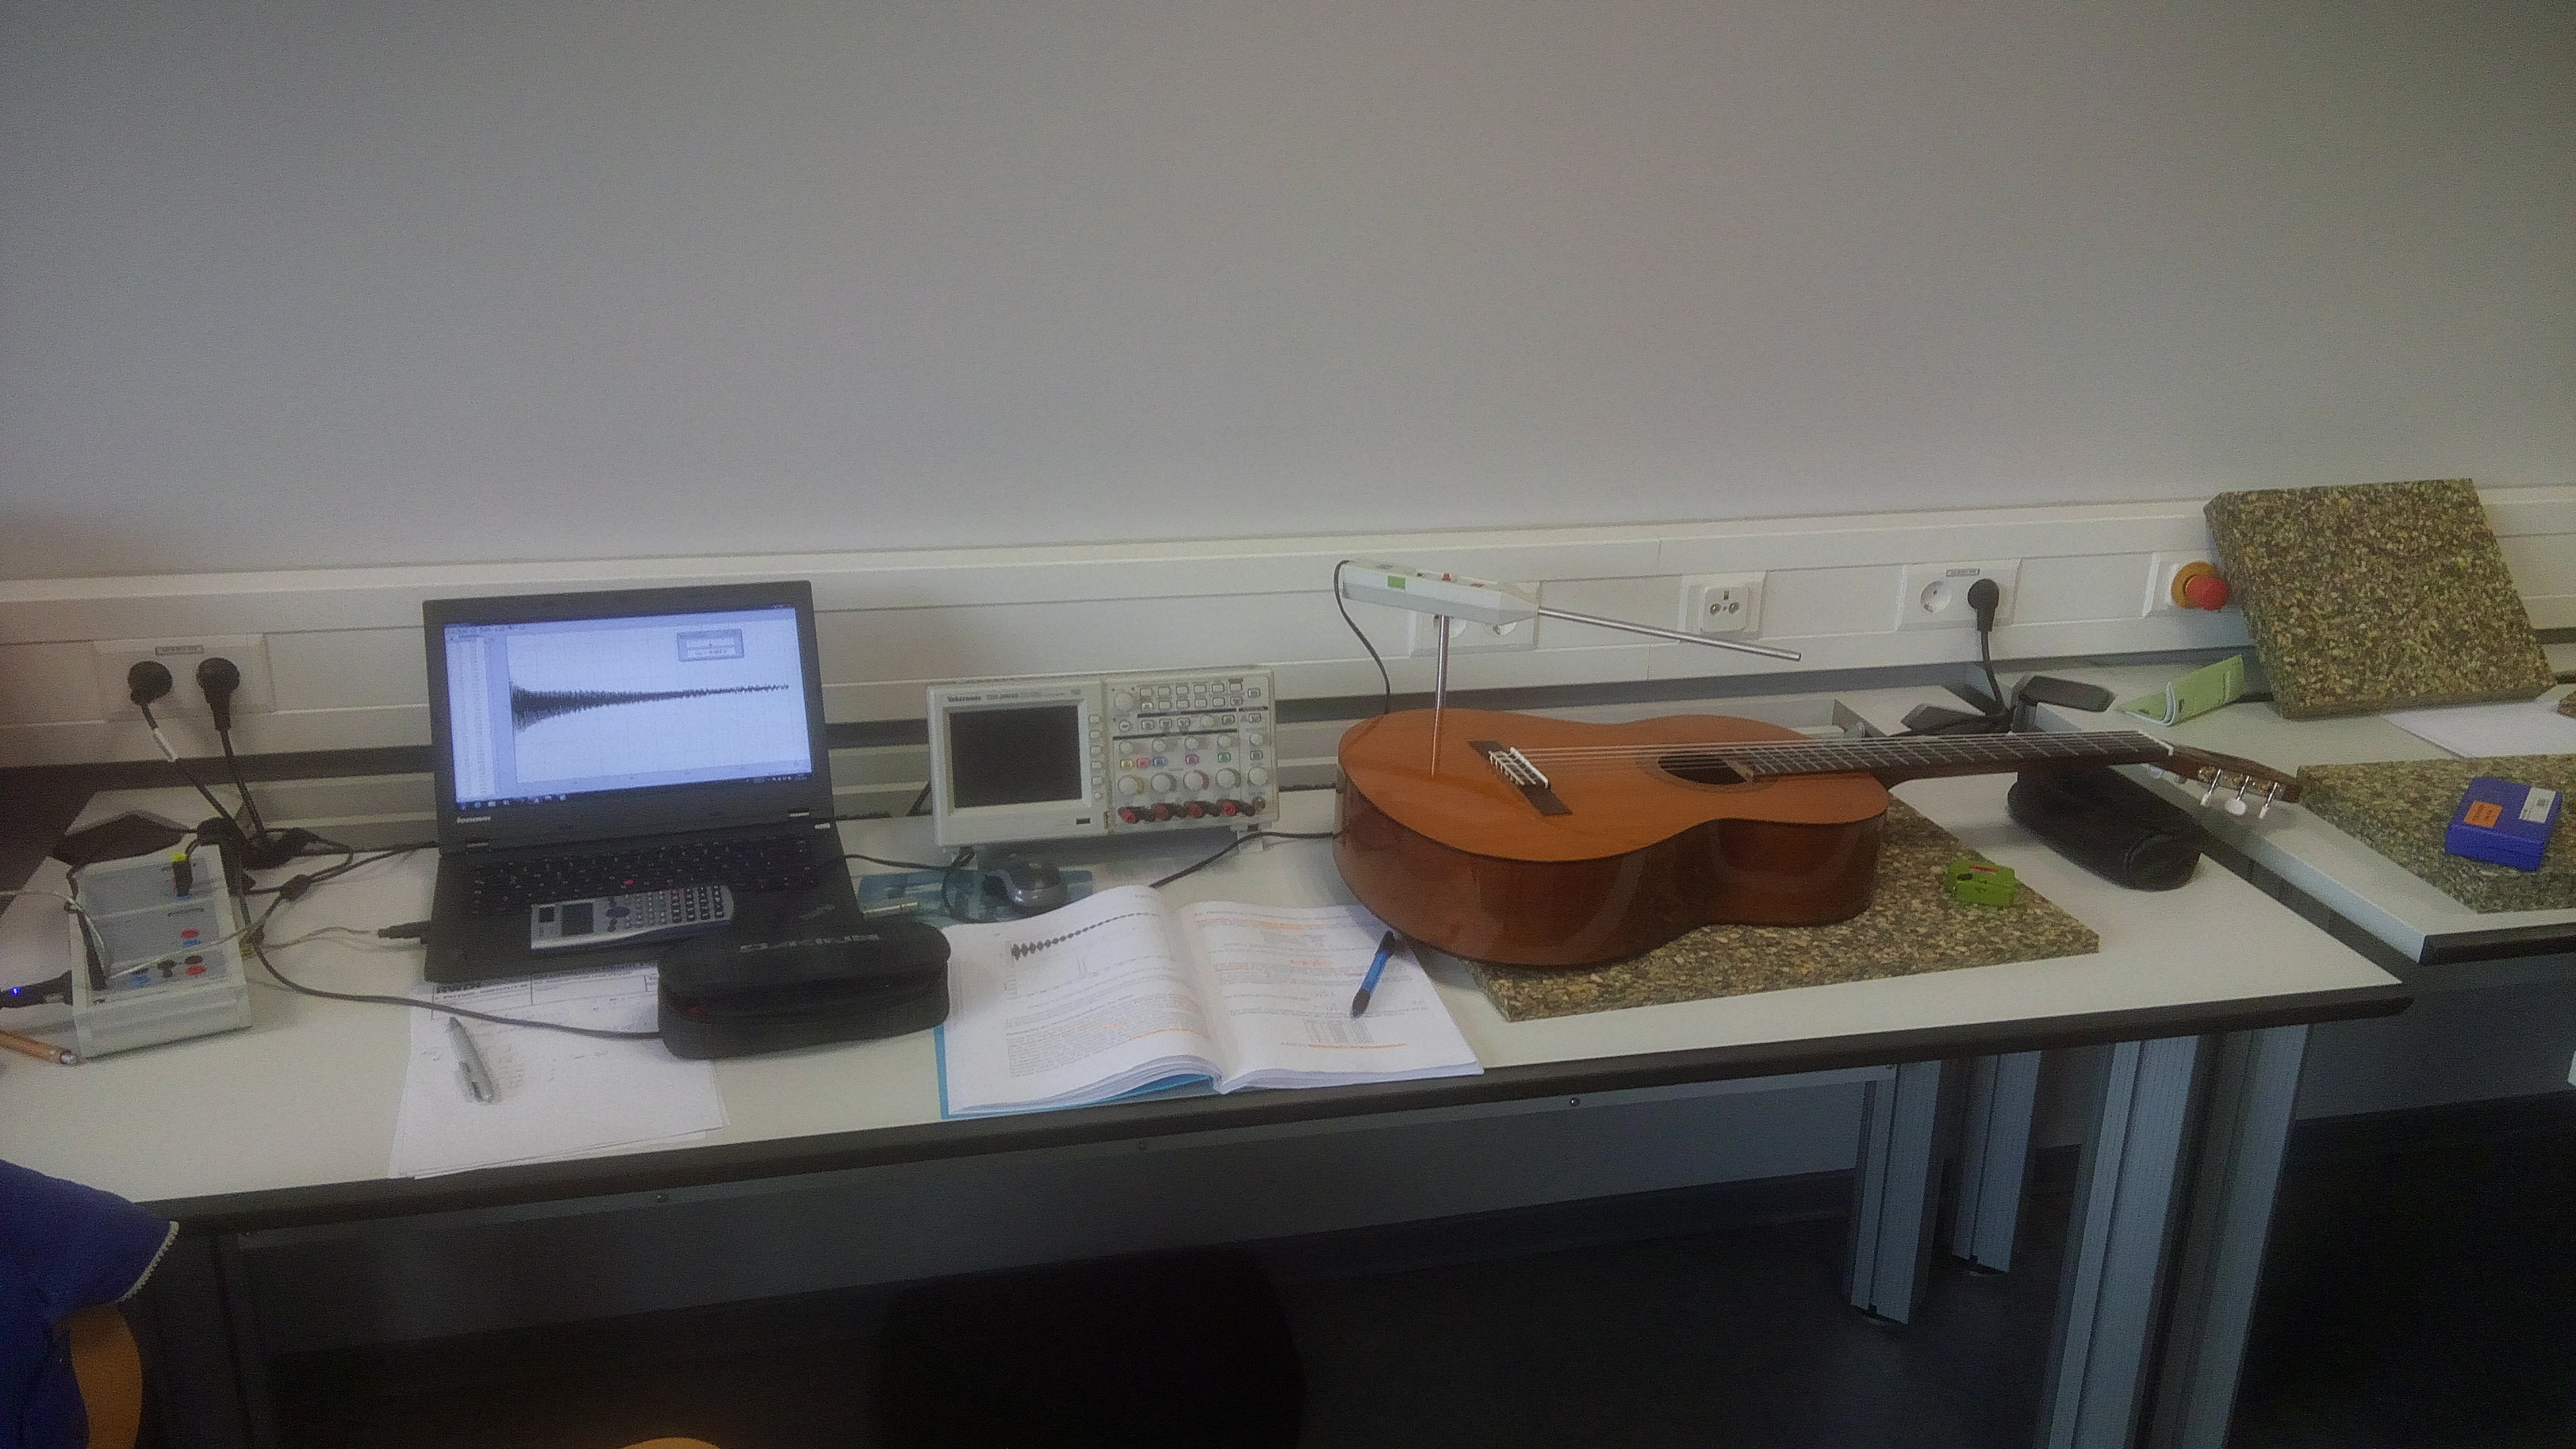
\includegraphics[scale=0.1]{Bilder/IMG_20160323_123920.jpg}
\caption{Versuchsaufbau für Messungen mit der Gitarre. }
\end{figure}


\begin{table}[H]\centering
\caption{Messparameter für Stimmversuche}
\begin{tabular}{c|c}
Parameter & Einstellungen \\ 
\hline
Messintervall & 500 $\mu s$ \\ 
Anzahl Messwerte & 10000 \\ 
Messdauer & 5s \\ 
Trigger & 0.3V \\ 
\end{tabular}
\end{table}
 

Wenn nun die D-Saite leer und die A-Saite im 5. Bund angeschlagen wurde, hörte man denselben Ton ohne Schwebung.

\begin{figure}[H]
\centering
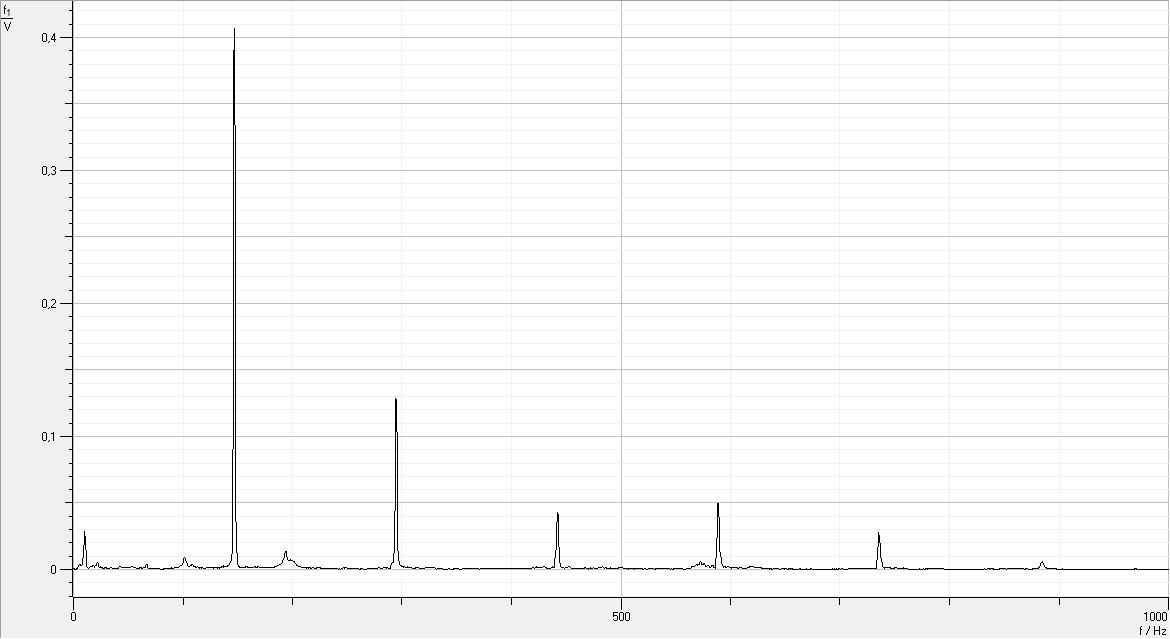
\includegraphics[scale=0.5]{Bilder/Gestimmt_Vorher.png}
\caption{D-Saite leer und A-Saite im 5. Bund nach dem Stimmen mit dem Stimmgerät. Es sind nur jeweils einzelne Peaks sichtbar also keine Schwebung.}
\end{figure}

Als Nächstes wurde die D-Saite so stark verstimmt, dass beim Anschlagen der D-Saite leer und A-Saite im 5. Bund eine deutliche Schwebung zu hören war.

\begin{figure}[H]
\centering
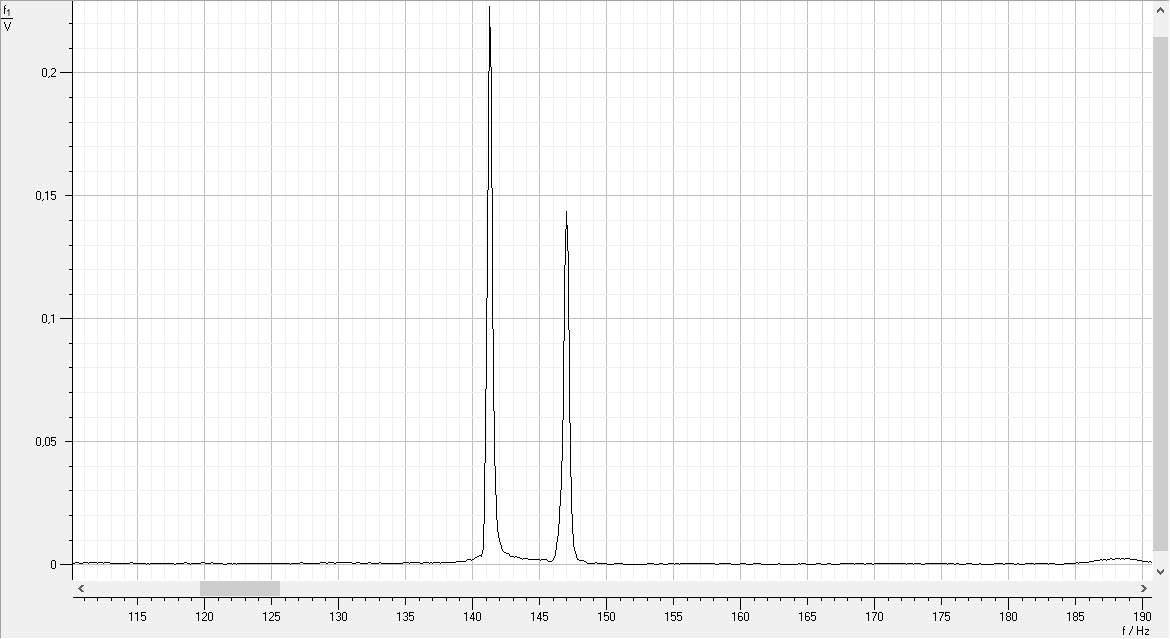
\includegraphics[scale=0.5]{Bilder/Verstimmt.png}
\caption{Verstimmte D-Saite leer und A-Saite im 5. Bund. Es ist eine deutliche Schwebung sichtbar.}
\end{figure}

Die jetzt verstimmte D-Saite wurde daraufhin so weit zurück gedereht bis die Schwebung wieder verschwand.

\begin{figure}[H]
\centering
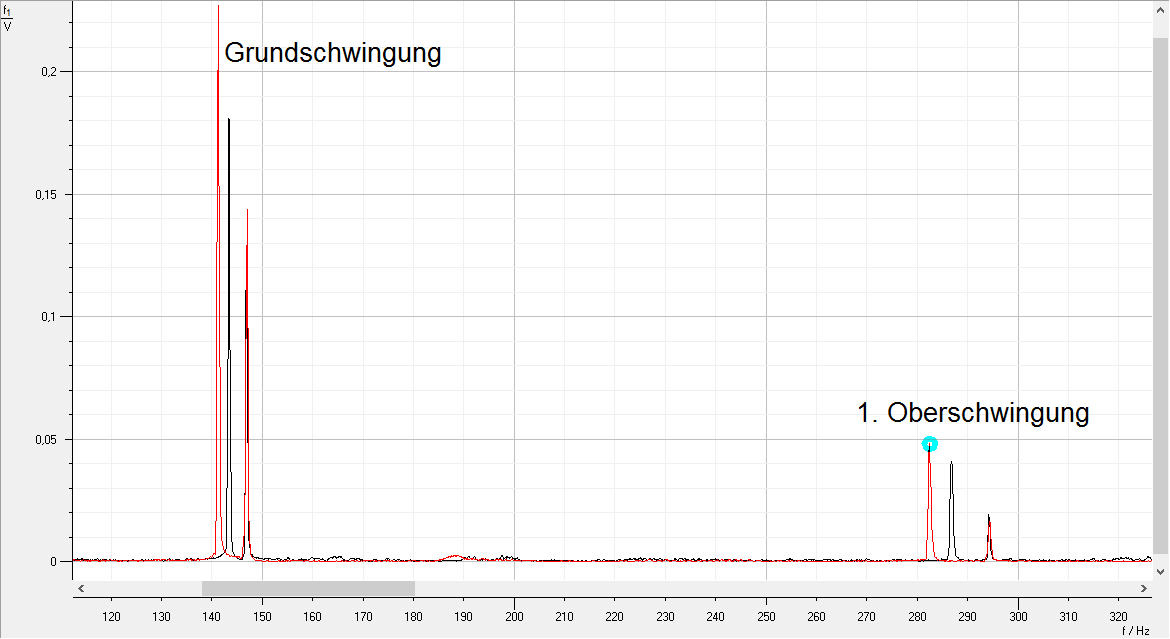
\includegraphics[scale=0.5]{Bilder/Verstimmt_vs_1_stimmen.png}
\caption{Verstimmte D-Saite in rot gegen den ersten Stimmversuch in schwarz. Die Peaks nähern sich. Besonders in der ersten Oberschwingung sieht man die Unterschiede noch deutlicher.}
\end{figure}

\begin{figure}[H]
\centering
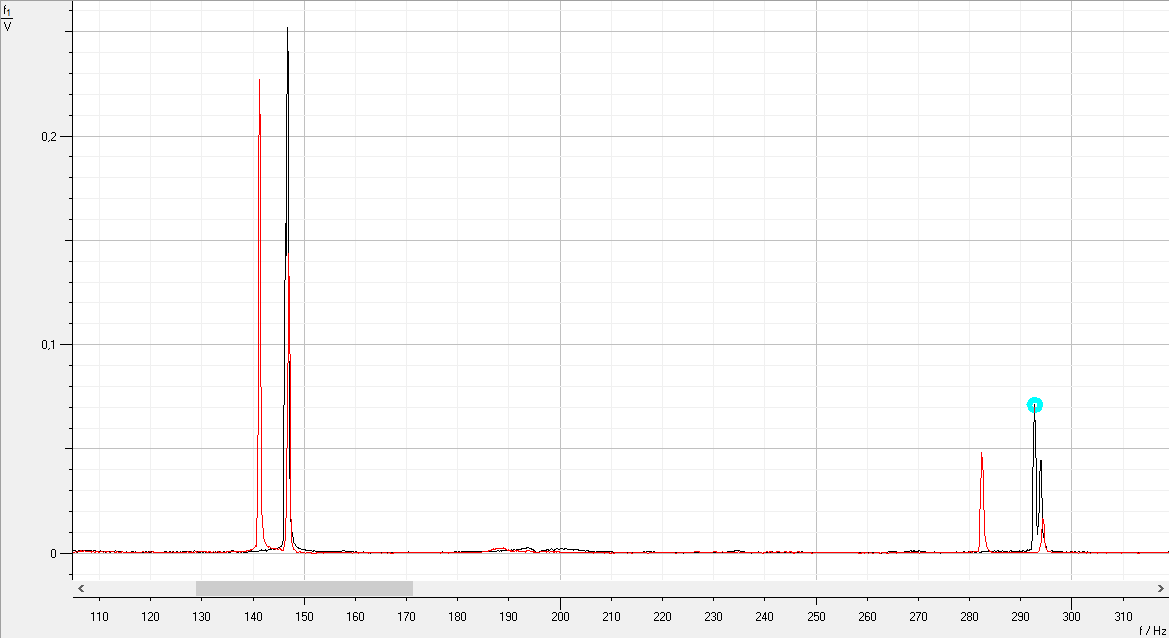
\includegraphics[scale=0.5]{Bilder/Verstimmt_vs_2_stimmen.png}
\caption{Verstimmte D-Saite in rot gegen den zweiten Stimmversuch in schwarz. Bei dem Peak der Grundschwingung ist schon keine Schwebung erkennbar aber in der 1. Oberschwingung sieht man noch eine leichte Schwebung.}
\end{figure}

\begin{figure}[H]
\centering
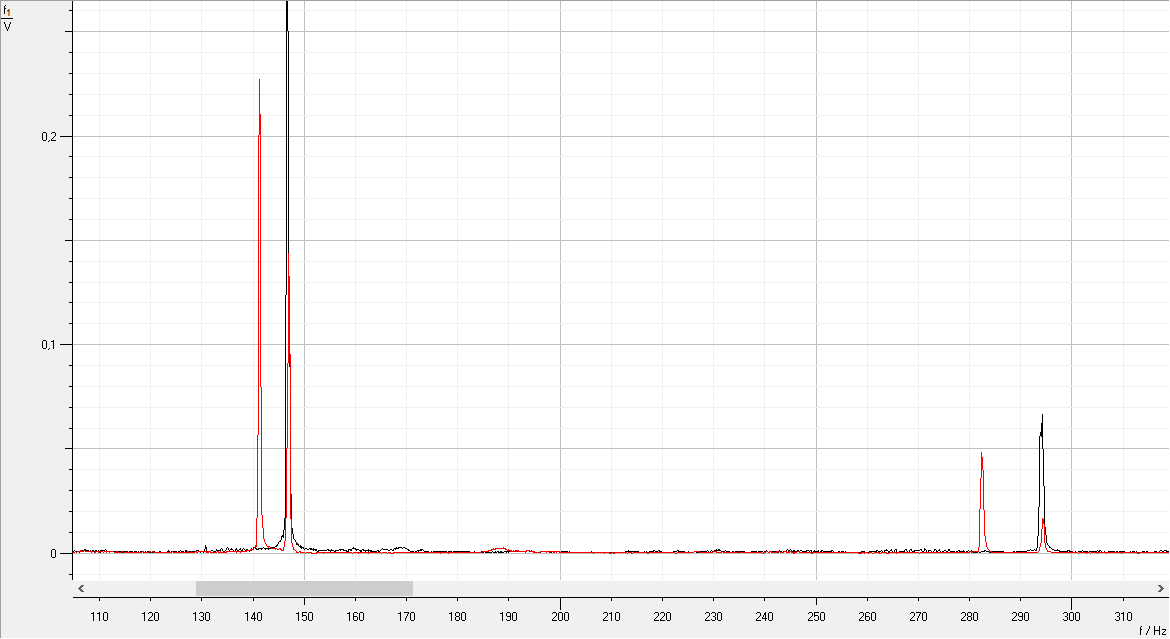
\includegraphics[scale=0.5]{Bilder/Verstimmt_vs_3_stimmen.png}
\caption{Verstimmte D-Saite in rot gegen den dritten Stimmversuch in schwarz. Bei den Peaks der Grundschwingung und der 1. Oberschwingung ist keine Schwebung erkennbar.}
\end{figure}

Die D-Saite sollte nun also wieder gut gestimmt sein, was auch mit dem Stimmgerät überprüft wurde. Das Stimmen über die Schwebung war also erfolgreich.

\section{Bestimmung der Materialeigenschaften der Saiten}
\subsection{Versuchsbeschreibung}
Für den Grundton $f$ einer Gitarrensaite gilt:
\begin{equation}
f=\frac{1}{2}\sqrt{\frac{T}{\mu}}\cdot \frac{1}{l}
\label{Grundgleichung Gitarre f gegen l}
\end{equation}
mit der Saitenspannung T in N, dem Massebelag $\mu$ in $\frac{kg}{m}$ und der Länge der Saite $l$ in m.
In diesem Versuch wird dieselbe Saite bei unterschiedlichen Längen angeschlagen und die entsprechende Frequenz gemessen. Trägt man dann $f$ gegen $\frac{1}{l}$ auf erhält man aus der Steigung $m=\frac{1}{2}\sqrt{\frac{T}{\mu}}$ einen Wert für das Verhältnis von $T$ und $\mu$, das mit den Herstellerangaben verglichen werden sollte.\newline Wir haben uns hier auf die Vermessung der Materialeigenschaften der A-Saite beschränkt.

\subsection{Versuchsaufbau und Durchführung}
Der Versuch wurde genau wie der erste Versuch mit der Gitarre aufgebaut. \newline
Zur Vermessung der Frequenz bei unterschiedlichen Längen wurde die A-Saite zuerst leer, dann im 2ten, 4ten, 6ten, 8ten und 10ten Bund jeweils 3 mal angeschlagen. Die Messung mit Mikrofon und Cassy selbst erfolgte wie im Teilversuch zuvor.
Die Frequenzen selbst wurden mittels Fast-Fourier-Transformation und Peakschwerpunktsberechnung bestimmt. Die jeweils drei Frequenzen wurden dann gemittelt und über Gleichung (\ref{sigmean}) der Fehler auf den Mittelwert bestimmt.
\newline
Die Länge der Anschlagpunkte wurden mit dem Maßband vermessen.\newline

\begin{table}[H]\centering
\caption{Messwerterfassungseinstellungen}
\begin{tabular}{c|c}
Parameter & Einstellung \\ 
\hline
Messintervall & 500 $\mu$s \\ 
Anzahl Messwerte & 10000 \\ 
Messdauer & 5s \\ 
Trigger & 0.3V \\ 
\end{tabular} 
\end{table}

\subsection{Versuchsauswertung}

\subsubsection{Rohdaten}
\begin{table}[H]\centering
\caption{Längenmessungen der Anschlagpunkte}
\begin{tabular}{c|c|c}
$L_0$ & 64.9 cm & Leere Saite\\ 
$L_1$ & 54.6 cm & 2. Bund \\ 
$L_2$ & 51.5 cm & 4. Bund \\ 
$L_3$ & 45.9 cm & 6. Bund \\ 
$L_4$ & 40.9 cm & 8. Bund \\ 
$L_5$ & 36.4 cm & 10. Bund \\ 
\end{tabular} 
\end{table}
Die Messung am 2. Bund wurde in der Auswertung ausgelassen, da die Längenmessung offenbar fehlgeschlagen ist. Die Abstände vom Steg zu den jeweiligen Bünden wurden mit dem Maßband bestimmt, daher haben wir den Fehler auf:
\begin{equation*}
\sigma_L=1 mm
\end{equation*}
abgeschätzt.


\begin{table}[H]\centering
\caption{Frequenzmessung bei unterschiedlichen Längen}
\begin{tabular}{c|cccccc}
 & $L_0$ & $L_1$ & $L_2$ & $L_3$ & $L_4$ & $L_5$ \\ 
\hline 
$f_1$ & 110.16 & 123.80 & 138.98 & 156.03 & 174.60 & 194.42 \\ 
$f_2$ & 110.20 & 123.79 & 139.04 & 155.69 & 174.31 & 196.00 \\ 
$f_3$ & 110.24 & 123.79 & 138.83 & 155.96 & 174.46 & 195.97 \\ 
$\bar{f}$ & 110.20 & 123.79 & 138.95 & 155.89 & 174.46 & 195.46 \\ 
$\sigma_{\bar{f}}$ & 0.02 & 0.00 & 0.06  & 0.10 & 0.08  & 0.52  \\ 
\end{tabular}
\newline 
Angaben in Hz
\end{table}
$~$\newline
Der Fehler auf die Frequenz ist bei der Vermessung des 2. Bunds sehr klein (ungerundet: $\sigma_{\bar{f_1}}=0.0033$). Dieser Wert wurde aber schon wegen der Längenmessung weggelassen.
$~$\newline
$~$\newline
Für die von uns vermessene A-Saite gilt laut Skript:
\begin{equation*}
\mu_{lit}=3.4095 \cdot 10^{-3} \frac{kg}{m}, \hspace{1cm}
T_{lit}=68.04 N.
\end{equation*}
Für die Steigung ist also ein Wert von
\begin{equation}
m_{lit}=\frac{1}{2}\sqrt{\frac{T_{lit}}{\mu_{lit}}}=70.633 \frac{m}{s}
\label{Herstellerangabe Gitarre}
\end{equation}
zu erwarten.
\subsubsection{Transformation der Rohdaten}
Die nun bestimmten gemittelten Frequenzen können jetzt mit ihren Fehlern gegen die jeweiligen Längen mit ihren Fehlern aufgetragen werden.
\begin{figure}[H]\centering
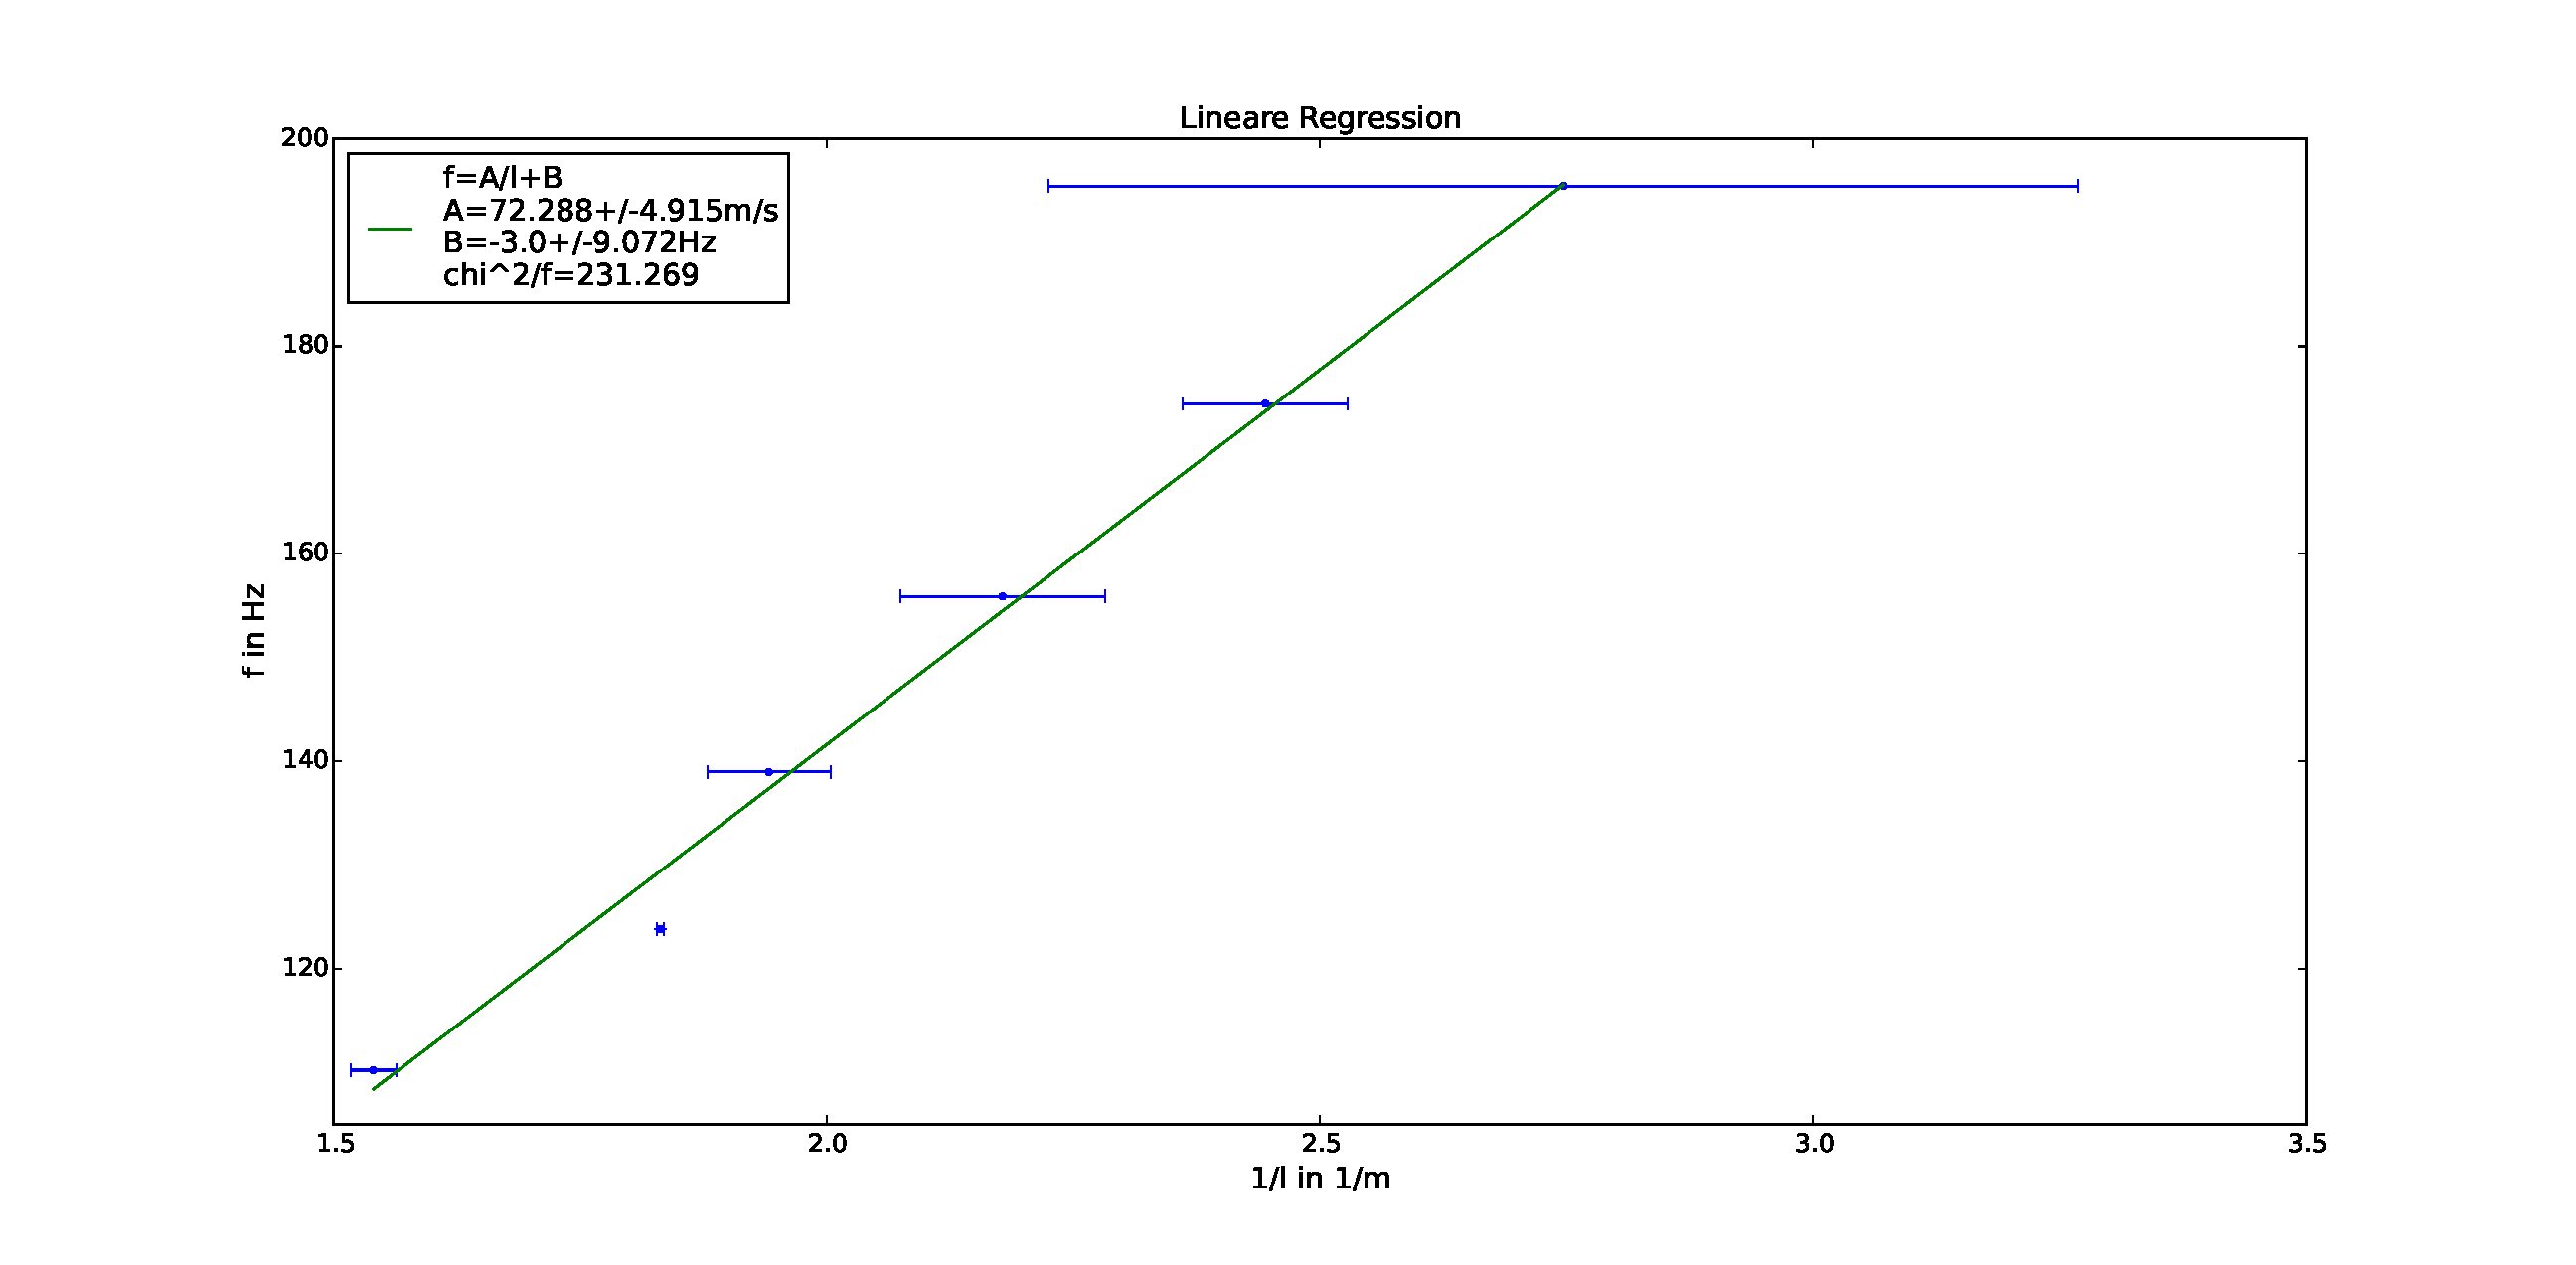
\includegraphics[scale=0.4]{Bilder/lin_reg_mit.eps}
\caption{Lineare Regression aller Werte. Der 2. Wert ist ein deutlicher Ausreißer und wurde daher im Folgenden weggelassen.}
\end{figure}

\begin{figure}[H]
\centering
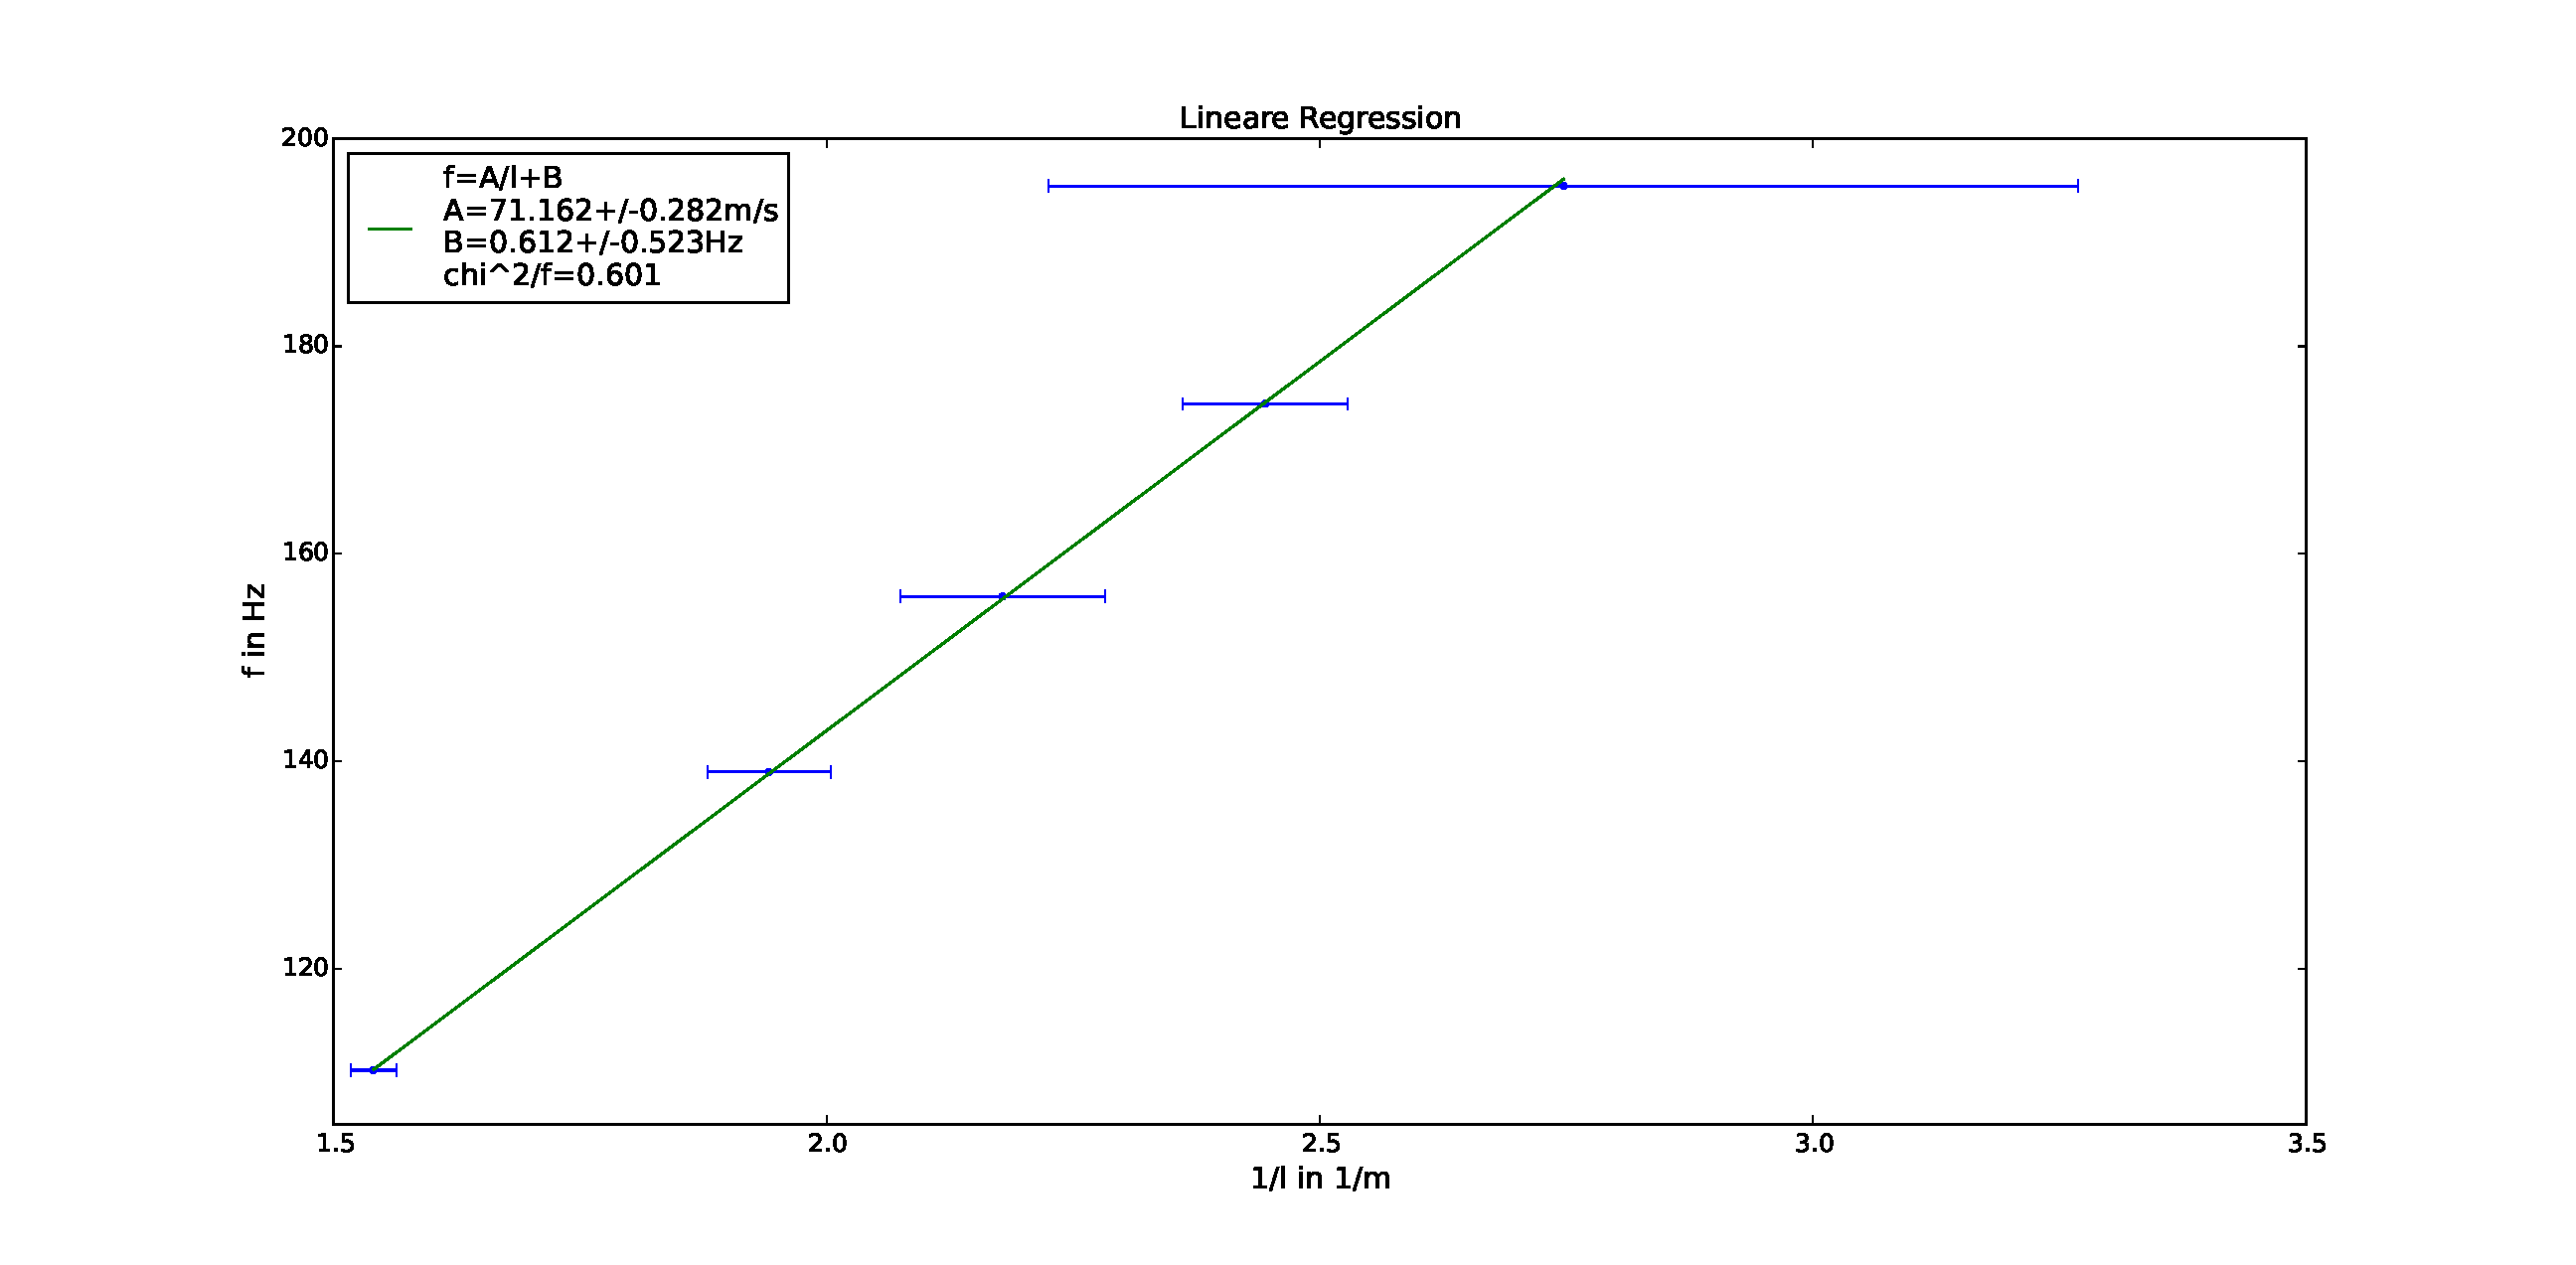
\includegraphics[scale=0.4]{Bilder/lin_reg_ohne.eps}
\caption{Lineare Regression ohne den zweiten Wert. Der Fehler steigt mit $\frac{1}{l}$, da die Saite bei kürzerer Länge stärker gedämpft ist und nicht so lange schwingt.}
\end{figure}


\begin{figure}[H]
\centering
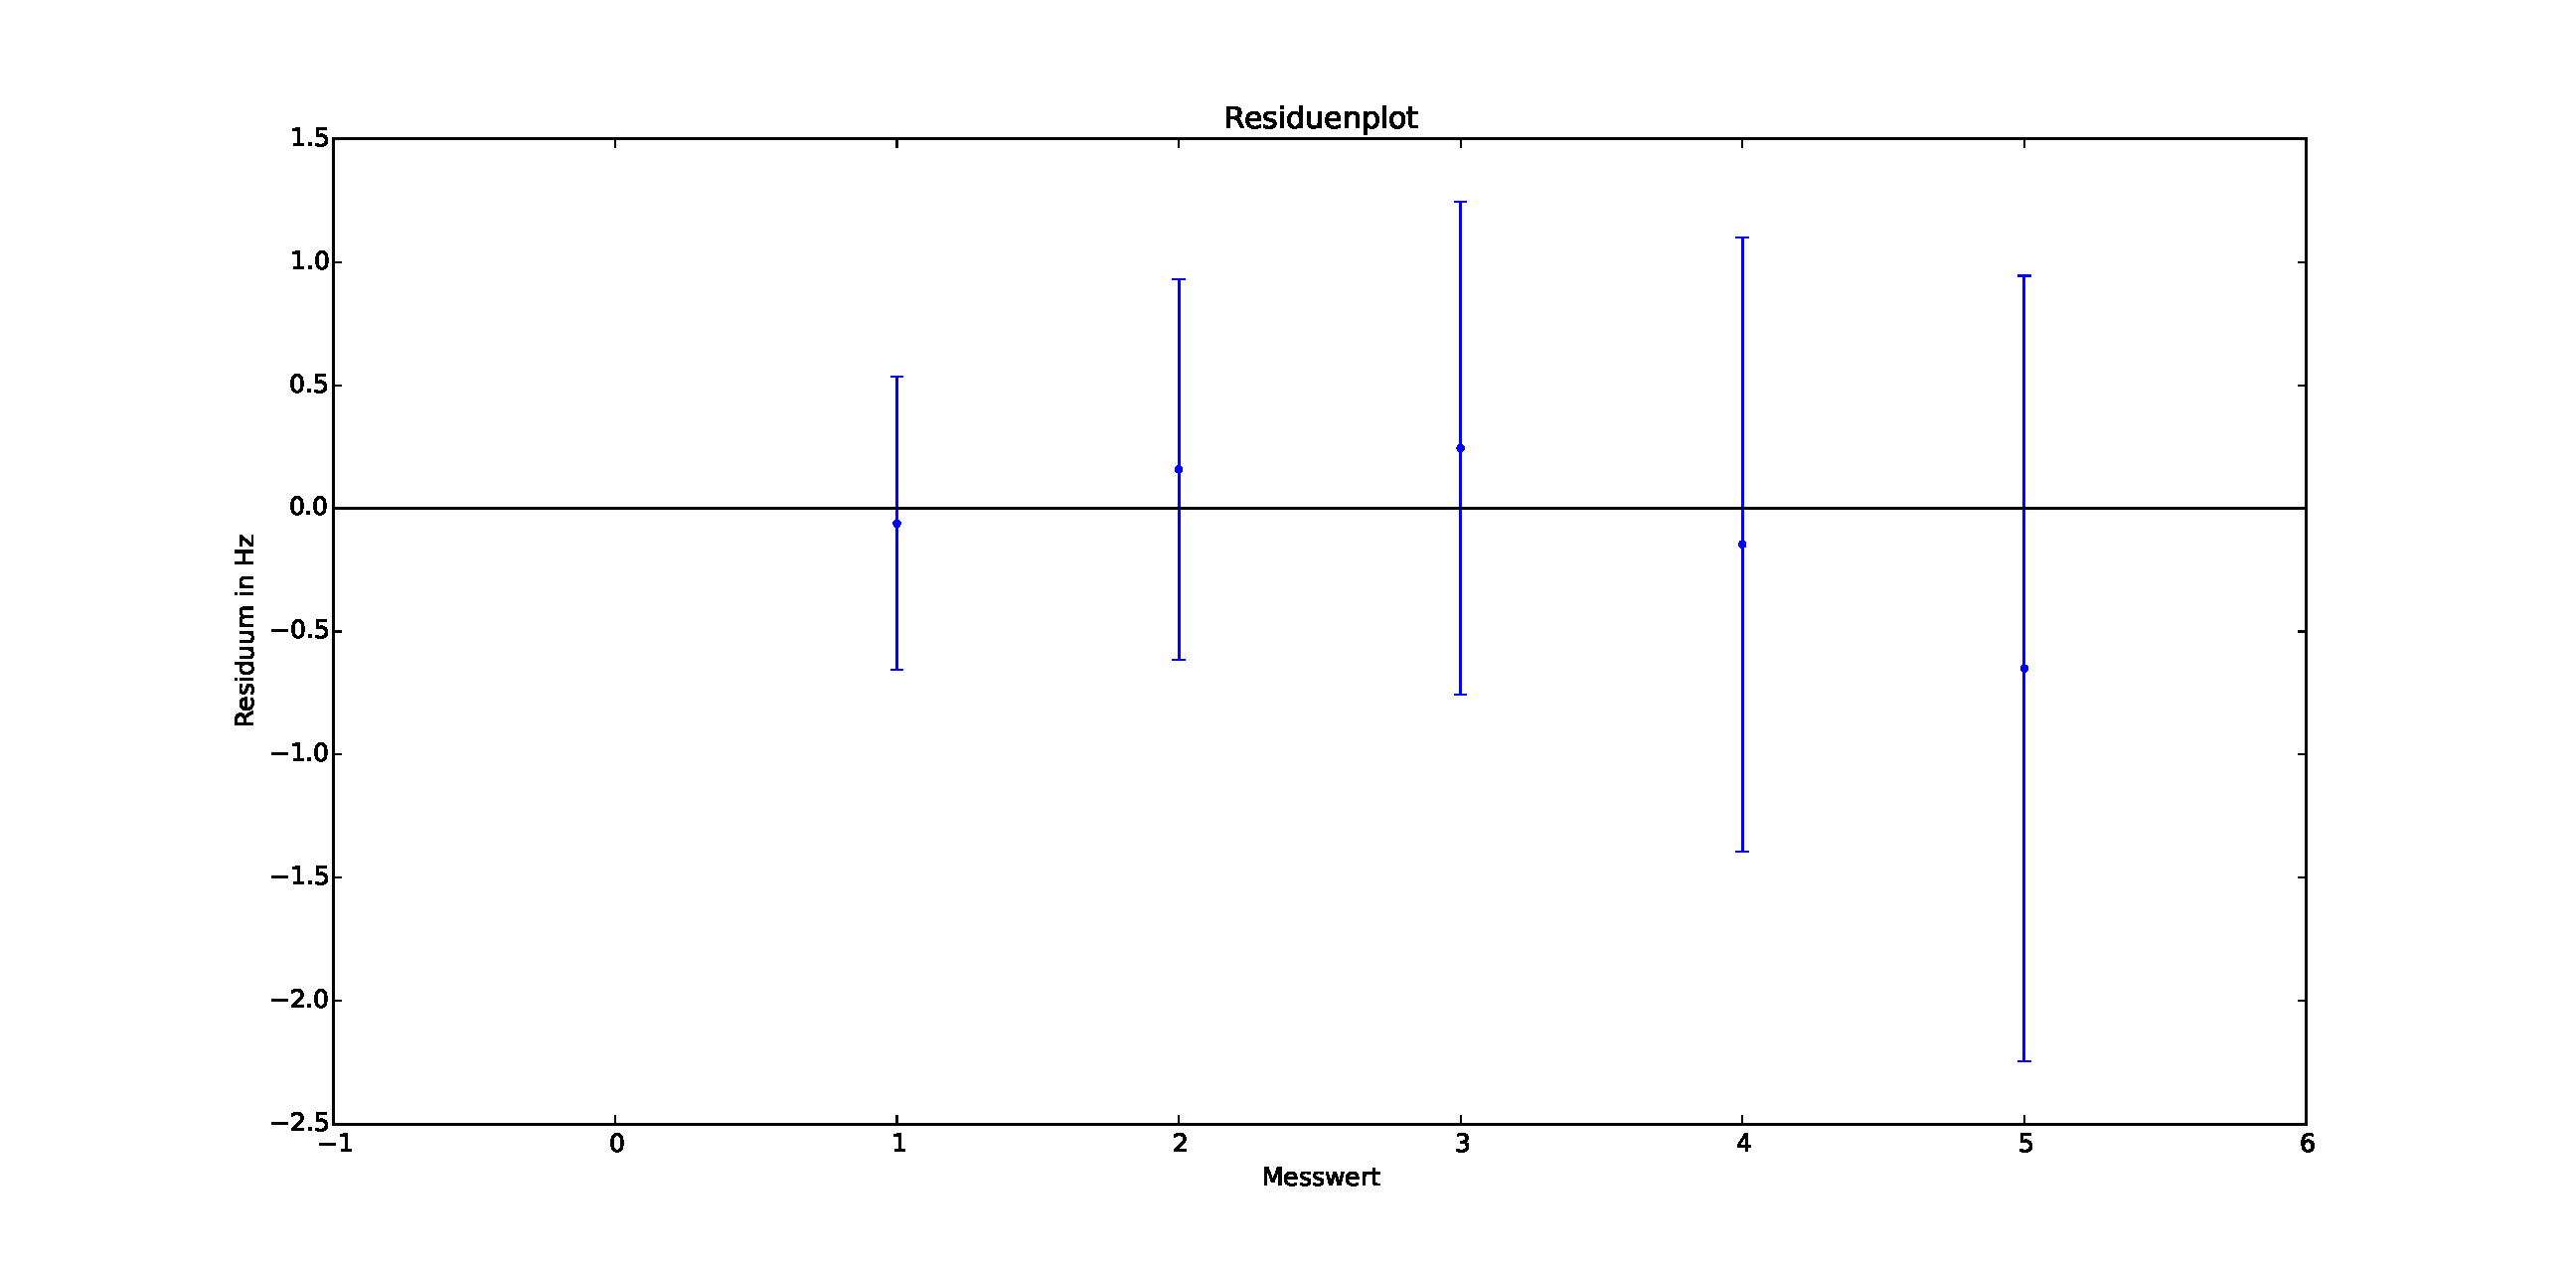
\includegraphics[scale=0.4]{Bilder/lin_reg_ohne_residuum.eps}
\caption{Residuenplot ohne den zweiten Wert. Der Residuenplot zeigt keine Systematik und alle Messwerte schneiden mit ihren Fehlern die Null-Linie.}
\end{figure}

Ergebnis der Linearen Regression:
\begin{align*}
A = m &= 71.162 \pm 0.282 \frac{m}{s}  \\
B &= 0.612 \pm 0.523 Hz \\
\frac{\chi^2}{f}&=0.601
\end{align*}

Zum Vergleich (siehe Gleichung \ref{Herstellerangabe Gitarre}):
\begin{equation}
m_{lit}=70.633 \frac{m}{s}
\end{equation}

\subsubsection{Fazit}
Der Wert aus den Herstellerangaben liegt im Bereich von 2 Standardabweichungen unter dem gemessenen Wert. Dies ist darauf zurückzuführen, dass die Gitarre im Laufe der Zeit abgenutzt wurde und daher der Massebelag mittlerweile eher kleiner ist als bei der Herstellerangabe für die neue Saite. \newline
Der gemessene y-Achsenabschnitt von $B = 0.612 \pm 0.523$ Hz liegt mit seinem Fehler nahe genug an dem erwarteten Wert von 0 (siehe Gleichung \ref{Grundgleichung Gitarre f gegen l}).
\newline
Das $\frac{\chi^2}{f}$ von 0.601 lässt zwar auf einen leicht überschätzten Fehler schließen, ist aber noch in einem vertretbaren Bereich.
\section{Aufnahme eines Frequenzspektrums}
\subsection{Versuchsbeschreibung}
Bei Grundschwingungen (1. Harmonische) befinden sich die Knoten an den Saiten-Enden. Neben der Grundschwingung bilden sich aber auch weitere sogenannte Oberschwingungen aus, die an den Enden ebenfalls Knoten bilden. Für die Wellenlängen dieser so genannten  n-ten Harmonischen gilt:
\begin{equation}
\lambda_n=	\frac{2L}{n}
\end{equation}
Für n=1 ergibt sich die Grundschwingung für n = 2 die 1. Oberschwingung für n = 3 die 2. Oberschwingung und so weiter.
\newline
\begin{figure}[H]
\centering
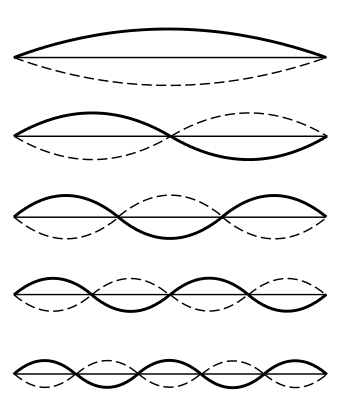
\includegraphics[scale=1]{Bilder/Harmonische.png}
\caption{Stehende Welle und deren Harmonische bis n = 5.}
\end{figure}

Schlägt man die Saite im Abstand $d=\frac{L}{n}$ an, fehlen die n-te Harmonische und ihre Vielfachen, da sich dort kein Knoten bilden kann.

In diesem Versuch sollte das Frequenzspektrum der D-Saite einer Gitarre, die an verschiedenen Abständen angeschlagen wurde auf das oben beschriebene Verhalten untersucht werden.

\subsection{Versuchsaufbau und Durchführung}
Der Aufbau ist derselbe wie in den anderen Versuchen zur Gitarre. 

\begin{table}[H]\centering
\caption{Messparameter für Aufnahme des Frequenzspektrums der D-Saite.}
\begin{tabular}{c|c}
Parameter & Einstellungen \\ 
\hline
Messintervall & 100 $\mu s$ \\ 
Anzahl Messwerte & 16000 \\ 
Messdauer & 1.6s \\ 
Trigger & 0.3V \\ 
\end{tabular}
\end{table}

Als Erstes wurde die D-Saite in der Mitte angeschlagen.
\begin{figure}[H]
\centering
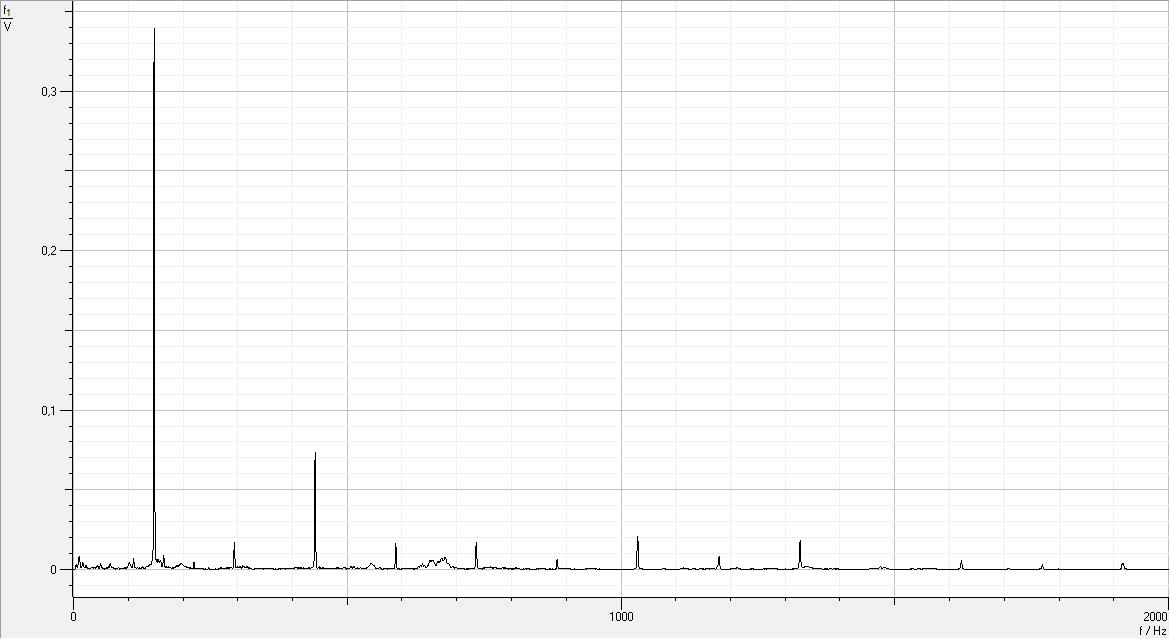
\includegraphics[scale=0.45]{Bilder/Spektrum_Mitte.png}
\caption{Grundfrequenz von 147,03 Hz ist deutlich erkennbar. Nur jede zweite Schwingung ist ausgeprägt.}
\end{figure}

Zum Vergleich wurde die Saite sehr weit oben am Hals angeschlagen.
\begin{figure}[H]
\centering
\includegraphics[scale=0.45]{Bilder/Spektrum_oben.png}
\caption{Die Amplituden fallen bis zur 6. Harmonischen stetig ab.}
\end{figure}

\subsection{Fazit}
Wie in den gezeigten Abbildungen zu sehen ist, konnten wir die Theorie, dass die n-ten Harmonischen fehlen, wenn man die Saite an einem Abstand von $d=\frac{L}{n}$ anschlägt, bestätigen.

\end{document}